\section{La radicación}

La potenciación también origina preguntas en sentido contrario. Si sabemos que
\[
3^2=9,
\]
podemos preguntar: ¿qué número elevado al cuadrado produce \(9\)? Esta pregunta puede escribirse como una ecuación:
\[
x^2=9.
\]
Buscar raíces consiste en recorrer el camino inverso: conocemos el exponente y el valor de la potencia, pero buscamos una base posible.

\subsection{Cuando los racionales no alcanzan}

Hasta ahora hemos ampliado nuestros conjuntos numéricos cuando las operaciones nos han llevado a cantidades que el conjunto disponible no podía representar. La radicación nos obligará a hacerlo nuevamente.

Consideremos un cuadrado de lado \(1\) como se ilustra en la figura \ref{fig:square}. Intuitivamente, el área de una figura mide cuánto espacio ocupa sobre el plano; en particular, un cuadrado de lado \(1\) tiene área \(1\). Más adelante estudiaremos estas ideas geométricas con mayor profundidad. Por ahora nos interesa otra medida del mismo cuadrado: la longitud de su diagonal.

\begin{figure}[!ht]
  \centering
  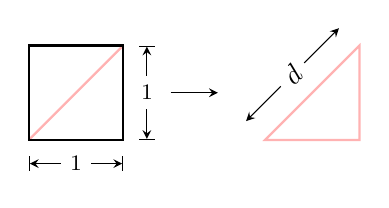
\begin{tikzpicture}[scale=1.2,>=stealth]
    \draw[thick,red!30] (0,0) -- (1,1);
    \draw[thick] (0,0) rectangle (1,1);
    \draw[|<->|] (0,-.25) -- node[fill=white,font=\footnotesize]{1} (1,-.25);
    \draw[|<->|] (1.25,0) -- node[fill=white,font=\footnotesize]{1} (1.25,1);

    \draw[->] (1.5,0.5) -- (2,0.5);

    \draw[thick,red!30] (2.5,0) -- (3.5,0) -- (3.5,1) -- cycle;
    \draw[<->] (2.3,.2) --node[sloped,fill=white]{\(d\)} ++(45:1.39);
  \end{tikzpicture}
  \caption{Representación de un cuadrado de lado uno y su diagonal}
  \label{fig:square}
\end{figure}

El teorema de Pitágoras, cuya justificación estudiaremos en geometría, permite relacionar los lados de un triángulo rectángulo. Aplicado al triángulo formado por dos lados del cuadrado y su diagonal \(d\), establece que
\[
d^2=1^2+1^2=2
\]

Por lo tanto, la diagonal debe ser un número positivo cuyo cuadrado sea \(2\).

Podemos preguntarnos entonces si alguna fracción representa exactamente esa longitud. Es decir, ¿existen enteros \(a\) y \(b\), con \(b\neq0\), tales que
\[
\left(\frac ab\right)^2=2?
\]

Supongamos que sí y que \(\frac ab\) está escrita en su forma irreducible. Entonces operamos sobre la expresión anterior, 
\begin{align*}
  \left(\frac ab\right)^2 &= 2 \\ 
  \frac{a^2}{b^2} &= 2 
\end{align*}
multiplicamos ambos miembros por \(b^2\):
\begin{align*}
  \frac{a^2}{b^2} b^2 &= 2b^2 \\
  \frac{b^2}{b^2} a^2 &= 2b^2 \\
  a^2&=2b^2
\end{align*}
Esto significa que \(a^2\) es par, ya que todo número multiplicado por \(2\) resulta ser un número par, y por lo tanto \(a\) también debe ser par. Podemos escribir \(a=2k\) para algún entero \(k\). Sustituyendo,
\[
(2k)^2=2b^2
\]
de donde
\[
4k^2=2b^2
\]
y, por tanto,
\[
b^2=2k^2
\]
Así, \(b^2\) también es par y, en consecuencia, \(b\) es par.

Pero entonces \(a\) y \(b\) tienen al menos un factor \(2\) en común, lo que contradice que \(\frac ab\) estuviera escrita en forma irreducible.

Por lo tanto, ningún número racional tiene cuadrado igual a \(2\).

Y aquí aparece algo importante. La diagonal del cuadrado no desaparece por el hecho de que ninguna fracción pueda representarla. Es una longitud perfectamente determinada por la figura; simplemente hemos descubierto que el conjunto \(\mathbb Q\) no contiene ningún número capaz de describirla exactamente.

Necesitamos entonces ampliar nuevamente nuestro sistema numérico.

Llamaremos \emph{números reales} a los números del conjunto \(\mathbb R\), que contiene a todos los racionales y también a números como el que representa la diagonal de este cuadrado. Este número se denota por
\[
\sqrt2.
\]
Por definición,
\[
\left(\sqrt2\right)^2=2,
\]
y acabamos de comprobar que
\[
\sqrt2\notin\mathbb Q.
\]

Los números reales que no son racionales reciben el nombre de \emph{irracionales}. Así,
\[
\sqrt2
\]
es un número irracional.

Una primera manera de imaginar \(\mathbb R\) es pensar en todos los números que pueden ubicarse sobre la recta numérica. Los racionales ocupan muchos de sus puntos, pero no todos. Los números irracionales permiten representar también aquellos puntos y longitudes que ninguna fracción puede describir exactamente.

De este modo,
\[
\mathbb N\subseteq\mathbb Z\subseteq\mathbb Q\subseteq\mathbb R.
\]

Construir rigurosamente el conjunto de los números reales requiere ideas que exceden nuestro propósito actual. Por ahora nos bastará una observación fundamental: una cantidad puede estar perfectamente determinada por un problema y, sin embargo, no pertenecer al conjunto numérico con el que veníamos trabajando. Cuando eso ocurre, necesitamos ampliar nuestro lenguaje numérico para poder representarla.

\begin{note}
Los números reales no son solamente objetos abstractos creados para hacer cálculos: aparecen de manera natural al describir numerosos fenómenos del mundo que nos rodea.

A medida que avance en el estudio de la matemática y la geometría encontrará algunos números especialmente importantes. Uno de ellos es
\[
\pi,
\]
llamado \emph{número pi} y representado mediante la letra griega pi minúscula. Aparece, por ejemplo, al estudiar circunferencias, áreas, ondas y movimientos periódicos.

Otro es
\[
e,
\]
conocido como \emph{número de Euler}. Surge de manera natural al estudiar procesos de crecimiento y decrecimiento continuo, como ciertos modelos de crecimiento poblacional, interés compuesto, fenómenos físicos y muchos otros procesos.

Estos números, junto con muchas de las ideas que irá aprendiendo, forman parte del lenguaje matemático utilizado para comprender la naturaleza y desarrollar gran parte de la ciencia y la tecnología modernas.
\end{note}

\subsection{Raíz \textit{n}-ésima}

Recapitulando lo que hemos visto; partimos de un número y de un exponente para calcular una potencia. Por ejemplo,
\[
2^3=8.
\]

Pero también podemos plantear el problema en sentido contrario:
\begin{center}
\textit{¿qué número elevado al cubo produce \(8\)?}
\end{center}
Como
\[
2^3=8,
\]
la respuesta es \(2\).

La radicación nace precisamente de esta pregunta. La expresión
\[
\sqrt[n]{a}
\]
se lee ``raíz \(n\)-ésima de \(a\)'' y busca un número que, elevado a \(n\), produzca \(a\).

En esta expresión, \(n\) recibe el nombre de \emph{índice} y \(a\) el de \emph{radicando}.

Por ejemplo,
\[
\sqrt[3]{8}=2
\]
porque
\[
2^3=8.
\]

Cuando el índice es \(2\), normalmente no se escribe:
\[
\sqrt a=\sqrt[2]{a}.
\]

Antes de definir con precisión qué valor representa una raíz, conviene observar algo que ya conocemos acerca de las potencias.

\subsection{¿Qué cambia si el índice es par o impar?}

Supongamos que queremos encontrar un número \(b\) que satisfaga
\[
b^n=a.
\]

Si \(b\) es positivo, su potencia será positiva cualquiera sea \(n\). La diferencia aparece cuando \(b\) es negativo.

Ya vimos que una cantidad par de factores negativos produce un resultado positivo, mientras que una cantidad impar produce un resultado negativo. Por ello,
\[
(-b)^n=
\begin{cases}
b^n, & \text{si \(n\) es par},\\
-b^n, & \text{si \(n\) es impar}.
\end{cases}
\]

Esta diferencia es la que determina el comportamiento de las raíces.

\subsubsection{Cuando el índice es impar}

Consideremos primero un índice impar, por ejemplo \(3\).

Tenemos
\[
2^3=8
\]
y también
\[
(-2)^3=-8.
\]

Al elevar a un exponente impar, el signo se conserva:
\[
\text{positivo}^{\text{impar}}=\text{positivo},
\qquad
\text{negativo}^{\text{impar}}=\text{negativo}.
\]

Por eso podemos buscar raíces impares tanto de números positivos como de números negativos:
\[
\sqrt[3]{8}=2,
\qquad
\sqrt[3]{-8}=-2.
\]

Además, elevar a una potencia impar no hace que un número y su opuesto produzcan el mismo resultado:
\[
2^3=8,
\qquad
(-2)^3=-8.
\]

De hecho, si aumentamos el número que usamos como base, también aumenta su potencia impar. Por ejemplo,
\[
1^3<2^3<3^3,
\]
y
\[
(-3)^3<(-2)^3<(-1)^3.
\]

Este comportamiento permite que cada número real tenga una única raíz real cuando el índice es impar.

Por lo tanto, si \(n\) es impar,
\[
\sqrt[n]{a}=b
\quad\Longleftrightarrow\quad
b^n=a.
\]

Por ejemplo,
\[
\sqrt[5]{32}=2
\]
porque
\[
2^5=32,
\]
mientras que
\[
\sqrt[5]{-32}=-2
\]
porque
\[
(-2)^5=-32.
\]

\subsubsection{Cuando el índice es par}

Veamos ahora qué ocurre con un índice par, por ejemplo \(2\).

Tenemos
\[
5^2=25,
\]
pero también
\[
(-5)^2=25.
\]

Esto sucede porque
\[
(-5)^2=(-5)(-5)=25.
\]

Lo mismo ocurre con cualquier exponente par: los factores negativos pueden agruparse de dos en dos y el resultado es no negativo.

Por ejemplo,
\[
(-2)^4=16,
\qquad
(-3)^6=729.
\]

Por lo tanto, ninguna potencia real de exponente par puede producir un número negativo.

Esto explica por qué una expresión como
\[
\sqrt{-4}
\]
no representa un número real: no existe ningún número real \(b\) que satisfaga
\[
b^2=-4.
\]

Si probamos con un número positivo,
\[
b^2>0,
\]
y si probamos con uno negativo, su cuadrado también es positivo. Finalmente,
\[
0^2=0.
\]
Ninguna de las posibilidades produce \(-4\).

En cambio, para un radicando positivo aparece otra cuestión.

Sabemos que
\[
5^2=25
\]
y
\[
(-5)^2=25.
\]

Por lo tanto, la ecuación
\[
b^2=25
\]
tiene dos soluciones reales:
\[
b=5
\qquad\text{y}\qquad
b=-5.
\]

Entonces podríamos preguntarnos:

\[
\text{¿qué valor debe representar \(\sqrt{25}\)?}
\]

Para que el símbolo radical represente una sola cantidad y no dos valores diferentes, se adopta la convención de elegir la solución no negativa.

Así,
\[
\sqrt{25}=5,
\]
y no \(\pm5\).

El número elegido recibe el nombre de \emph{raíz principal}.

En general, si \(n\) es par y \(a\ge0\),
\[
\sqrt[n]{a}=b
\]
significa que
\[
b^n=a
\qquad\text{y}\qquad
b\ge0.
\]

Por lo tanto,
\[
\sqrt[4]{16}=2,
\]
aunque también sea cierto que
\[
(-2)^4=16.
\]

La expresión
\[
\sqrt[4]{16}
\]
representa solamente la raíz principal, es decir, \(2\).

\begin{note}
Hay una diferencia importante entre
\[
\sqrt{25}=5
\]
y resolver la ecuación
\[
x^2=25.
\]

El radical \(\sqrt{25}\) representa, por definición, una sola cantidad: la raíz principal no negativa.

En cambio, al resolver
\[
x^2=25,
\]
debemos buscar todos los números cuyo cuadrado sea \(25\). Por eso las soluciones son
\[
x=5
\qquad\text{y}\qquad
x=-5.
\]
\end{note}

La existencia de raíces \(n\)-ésimas para todos los números reales permitidos puede demostrarse rigurosamente a partir de propiedades más profundas de los números reales. Por ahora nos concentraremos en comprender cómo se comportan y cómo operar con ellas.

\subsection{El radical representa un solo número}

Es importante distinguir una raíz de las soluciones de una ecuación.

Por ejemplo,
\[
\sqrt{25}=5.
\]

El símbolo \(\sqrt{\phantom a}\) representa una sola cantidad. Como se trata de una raíz de índice par, elegimos por definición la raíz no negativa.

Sin embargo, si preguntamos
\[
\text{¿qué números elevados al cuadrado producen \(25\)?}
\]
encontramos dos respuestas:
\[
5^2=25
\]
y
\[
(-5)^2=25.
\]

Por lo tanto, la ecuación
\[
x^2=25
\]
tiene dos soluciones:
\[
x=5
\qquad\text{o}\qquad
x=-5.
\]

Podemos escribirlas de manera abreviada como
\[
x=\pm5.
\]

El signo \(\pm\) no forma parte del valor de
\[
\sqrt{25}.
\]
Aparece porque estamos reuniendo las dos soluciones posibles de la ecuación.

Así,
\[
\boxed{\sqrt{25}=5}
\]
pero
\[
\boxed{x^2=25\quad\Longrightarrow\quad x=\pm5}.
\]

Hay una razón por la que debemos tener este cuidado. Al elevar un número a un exponente par, su signo puede dejar de distinguirse:
\[
3^2=9
\qquad\text{y}\qquad
(-3)^2=9.
\]

Una vez obtenido el \(9\), ya no podemos saber solamente a partir de ese resultado si el número original era \(3\) o \(-3\).

Por ahora evitaremos utilizar la raíz como una operación mecánica para ``deshacer'' potencias dentro de ecuaciones. Más adelante estudiaremos herramientas que nos permitirán hacerlo de manera segura.

En cambio, cuando simplemente calculamos una expresión como
\[
\sqrt{36},
\]
no existe ambigüedad:
\[
\sqrt{36}=6.
\]

El radical representa siempre el valor principal que hemos definido.


\subsection{Algoritmo para aproximar raíces}

Algunas raíces pueden reconocerse inmediatamente:
\[
\sqrt{25}=5
\]
porque
\[
5^2=25,
\]
o
\[
\sqrt[3]{125}=5
\]
porque
\[
5^3=125.
\]

Pero no siempre ocurre esto.

Consideremos, por ejemplo,
\[
\sqrt{17}.
\]

Estamos buscando un número cuyo cuadrado sea \(17\). No parece haber un número entero que lo produzca exactamente, pero podemos comenzar buscando entre qué números se encuentra.

Sabemos que
\[
4^2=16
\]
y
\[
5^2=25.
\]

Como
\[
16<17<25,
\]
la raíz debe encontrarse entre \(4\) y \(5\):
\[
4<\sqrt{17}<5.
\]

Ahora podemos investigar los décimos.

Probemos con \(4{,}1\):
\[
4{,}1^2=16{,}81.
\]

Todavía estamos por debajo de \(17\).

Probemos con \(4{,}2\):
\[
4{,}2^2=17{,}64.
\]

Ahora nos hemos pasado. Por lo tanto,
\[
4{,}1<\sqrt{17}<4{,}2.
\]

Podemos continuar de la misma manera con los centésimos:
\[
4{,}12^2=16{,}9744,
\]
mientras que
\[
4{,}13^2=17{,}0569.
\]

Entonces,
\[
4{,}12<\sqrt{17}<4{,}13.
\]

Si necesitamos mayor precisión, podemos repetir nuevamente el procedimiento:
\[
4{,}123^2=16{,}999129,
\]
mientras que
\[
4{,}124^2=17{,}007376.
\]

Así,
\[
4{,}123<\sqrt{17}<4{,}124.
\]

Podemos continuar tanto como sea necesario.

Este procedimiento nos proporciona aproximaciones cada vez mejores:
\[
\sqrt{17}\approx4{,}123.
\]

Observe que
\[
\sqrt{17}
\]
y
\[
4{,}123
\]
no significan exactamente lo mismo. El radical representa el número exacto; el decimal es solamente una aproximación.

\subsubsection{Un procedimiento general}

Para aproximar una raíz \(n\)-ésima podemos proceder de la siguiente manera:

\begin{enumerate}
    \item Buscamos dos números entre cuyas potencias \(n\)-ésimas se encuentre el radicando.
    \item Con ello sabemos entre qué dos números se encuentra la raíz.
    \item Probamos valores intermedios para estrechar el intervalo.
    \item Repetimos el procedimiento hasta alcanzar la precisión que necesitemos.
\end{enumerate}

Por ejemplo, para aproximar
\[
\sqrt[3]{390},
\]
comenzamos observando que
\[
7^3=343
\]
y
\[
8^3=512.
\]

Como
\[
343<390<512,
\]
sabemos que
\[
7<\sqrt[3]{390}<8.
\]

Probemos ahora con décimos:
\[
7{,}3^3=389{,}017,
\]
mientras que
\[
7{,}4^3=405{,}224.
\]

Por tanto,
\[
7{,}3<\sqrt[3]{390}<7{,}4.
\]

Podemos seguir probando centésimos y milésimos si necesitamos una aproximación más precisa.

No todas las raíces producen un número sencillo que podamos reconocer de inmediato. En esos casos, conservar el radical,
\[
\sqrt{17},
\]
nos permite representar el valor de manera exacta, mientras que una escritura como
\[
4{,}123
\]
nos proporciona una aproximación útil.

\begin{note}
Es normal sentir que expresiones como
\[
\sqrt{17}
\qquad\text{o}\qquad
\sqrt[3]{390}
\]
son cálculos que todavía deben ``resolverse''. Sin embargo, el radical ya representa un número.

Cuando una raíz puede reconocerse exactamente, escribimos su valor:
\[
\sqrt{25}=5.
\]
Pero si no existe un valor sencillo que podamos reconocer, no es necesario reemplazar la raíz por una aproximación decimal. En matemáticas suele preferirse conservar la expresión exacta:
\[
\sqrt{17}.
\]

Una escritura decimal como
\[
\sqrt{17}\approx4{,}1231
\]
es solamente una aproximación y se utiliza cuando el problema requiere conocer un valor numérico aproximado.

Actualmente, calculadoras y computadoras pueden obtener aproximaciones con una precisión enorme utilizando algoritmos numéricos que refinan progresivamente el resultado. El procedimiento de acotar la raíz que hemos visto comparte esa misma idea general: comenzar con información aproximada e ir acercándose cada vez más al valor buscado.

Por ahora, lo más importante es recordar que
\[
\boxed{\sqrt{17}\text{ ya es un número}}
\]
y constituye una respuesta exacta. No necesita transformarlo en un decimal a menos que el problema lo solicite o que una aproximación resulte útil para el cálculo que está realizando.
\end{note}
